
\begin{document}
\setcounter{chapter}{0}

\chapter{Velocity}

\begin{tcolorbox}[enhanced,colback=white,colframe=teal,sharp corners,boxrule=1pt,
  title=\textbf{In this chapter},coltitle=white,colbacktitle=teal,left=3mm,right=3mm]
By the end of this chapter you should be able to
\begin{itemize}[itemsep=2pt,topsep=2pt]
  \item explain what a \emph{conceptual model} is, why every model is a simplification, and how scientists decide whether a model can be trusted;
  \item draw and read a \emph{dot diagram}, rank objects by speed from the spacing of their dots, and explain why the time between dots must be the same for every diagram you compare;
  \item define \emph{speed} two ways: as distance divided by time, and as the \emph{rate of change} of position; recover distance from speed two ways: as speed times time, and as the \emph{area} under a speed--time graph;
  \item distinguish \emph{average speed} from \emph{instantaneous speed}, read both from a position--time graph, and explain in what sense a speedometer reading is a limit;
  \item convert between metres per second, kilometres per hour, and miles per hour, and carry units through a calculation so that they check the answer;
  \item follow how a footprint's stride length and foot length were turned into a speed estimate, and identify the assumptions hidden in each step;
  \item perform a \emph{sanity check} on the output of a model, recognise \emph{extrapolation} beyond the data a model was built from, and explain why it is dangerous;
  \item report a result with an \emph{uncertainty}, convert between absolute and percentage uncertainty, and propagate an uncertainty through a simple formula;
  \item distinguish \emph{speed} from \emph{velocity} and \emph{distance} from \emph{displacement}, and compute average velocity along a line with the correct sign.
\end{itemize}
\end{tcolorbox}

\begin{tcolorbox}[enhanced,colback=slatepale,colframe=slate,sharp corners,boxrule=0.6pt,
  title=\textbf{How to read this chapter: two perspectives},coltitle=white,colbacktitle=slate,left=3mm,right=3mm]
Every idea in this book can be understood with elementary mathematics alone: ratios, averages, and the areas of simple shapes. Every idea can also be understood with calculus, the mathematics of rates of change, which was invented largely to describe motion. Neither view is the ``real'' one; each illuminates the other. Throughout, explanations and solutions are labelled
\begin{center}
\elemtag\quad for the route using only elementary mathematics, and \qquad \calctag\quad for the route using derivatives and integrals.
\end{center}
If you have not yet met derivatives and integrals, read the \elemtag\ route and skip the other; nothing later in the chapter depends on it. If you have met them, read both, and check that they agree. The calculus in this chapter is gentle, because speed is the simplest rate there is; Chapter~2 will lean on it harder.
\end{tcolorbox}

\section{An Ancient Sprinter}

In 2003, in the dry lake country of western New South Wales, Australia, a young Mutthi Mutthi woman named Mary Pappin noticed a mark in the hard clay of an old lakebed. It was a human footprint. Archaeologists who followed up the discovery uncovered hundreds more: trackways left by adults and children who had walked and run across the wet margin of a lake in the Willandra Lakes region, and whose prints had dried, been buried, and survived. Dating by a technique called optically stimulated luminescence, which measures how long mineral grains in the sediment have been hidden from sunlight, placed the prints at roughly \num{19000} to \num{23000} years old. They are among the oldest human footprints known anywhere.

One set of prints attracted particular attention. A team of Pintubi trackers, who read footprints for a living, examined the site and concluded that most of the tracks were made by people walking, some in family groups, but that a few were made by hunters moving fast, apparently to cut off an animal's escape. One hunter had been running very hard.

The scientist leading the excavation, Steve Webb, wanted to say \emph{how} hard. He measured the prints with a tape measure, did some arithmetic, and arrived at a running speed of just over \SI{10}{\metre\per\second}. That is roughly the average speed of the world's best sprinters over \SI{100}{\metre}. Newspapers put it more colourfully: a barefoot hunter running through mud twenty thousand years ago could have kept pace with Usain Bolt. The story travelled around the world.

And then, a few years later, it quietly went away.

How did Webb turn a footprint into a speed? What did his calculation assume, and where did it go wrong? What is the hunter's speed, as best we can now tell? Answering those questions is the business of this chapter, and along the way we will meet the ideas that the rest of the book is built on: \emph{models}, \emph{dot diagrams}, \emph{speed}, \emph{uncertainty}, and \emph{velocity}.

\section{Models in Science}

Webb did not use any high-technology equipment to estimate the hunter's speed, and he did not rely on the trackers' judgement either. He made a few measurements and fed them into a \emph{conceptual model}.

\begin{definition}{Conceptual model}{model}
A \textbf{conceptual model} is a deliberately simplified way of thinking about one particular part of the world. It may combine measurements, diagrams, equations, graphs, tables of data, and computer programs. A model is never a complete description of the thing it models; it keeps the features that matter for the question at hand and leaves out everything else. A good model is one whose simplifications do not spoil the answer to the question you are asking.
\end{definition}

A road map is a model. It leaves out the colour of the houses, the height of the trees, and the weather, and it shrinks everything by a factor of fifty thousand, but for the question ``how do I drive from here to the coast?'' those omissions cost nothing. Use the same map to decide where to plant a garden and it fails, not because it is wrong but because it was built for a different question.

Physics is full of models, and much of learning physics is learning which model fits which question. In this chapter we will build a model of running from footprints. In later chapters we will model a falling stone as a point with no air around it, a planet as a sphere, and a bridge as a set of rigid rods. Every one of these is false in some respect, and every one is useful.

\begin{modelnote}[Facts, hypotheses, and sanity checks]
Hewitt describes science as resting less on a fixed recipe than on an \emph{attitude}: inquiry, integrity, and a willingness to admit error. In that spirit, a scientific \emph{fact} is a close agreement among competent observers about something they have all measured, and a \emph{hypothesis} is an educated guess that stays provisional until experiment supports it. The crucial test of whether a hypothesis is scientific at all is whether some observation \emph{could} show it to be wrong. As Einstein put it, no number of experiments can prove a claim right, but a single experiment can prove it wrong.

A model's output is a hypothesis about the world, and it deserves the same treatment. If a model says a Stone Age hunter ran as fast as an Olympic champion, the scientific response is not to be impressed but to ask what \emph{else} the model predicts and whether those predictions survive comparison with things we already know. We will do exactly that in Section~\ref{sec:questioning}, and we will call it a \emph{sanity check}.
\end{modelnote}

\section{From Footprints to Dot Diagrams}
\label{sec:dots}

\subsection{What Webb measured}

Look at a line of footprints left by someone walking or running in a straight line. The prints alternate: left, right, left, right. They do not lie exactly on one line, because the left foot lands a little to the left of the direction of travel and the right foot a little to the right. Figure~\ref{fig:footprints} shows the pattern.

Webb measured two things. The first was the \textbf{stride length}: the distance from one print of the right foot to the \emph{next} print of the right foot. One stride is two steps. The second was the \textbf{foot length}: the length of a single print, heel to toe. We will see in Section~\ref{sec:stridemodel} why the foot length mattered to him.

\begin{figure}[htb]
\centering
\begin{tikzpicture}[x=1cm,y=1cm]
  % right-foot prints (upper row) and left-foot prints (lower row)
  \foreach \x in {0,3.6,7.2}{
    \begin{scope}[shift={(\x,0.55)}]
      \fill[slate!60,rotate=-8] (0,0) ellipse (0.42 and 0.17);
      \fill[slate!60,rotate=-8] (0.36,0.06) ellipse (0.13 and 0.11);
    \end{scope}}
  \foreach \x in {1.8,5.4,9.0}{
    \begin{scope}[shift={(\x,-0.55)}]
      \fill[slate!60,rotate=8] (0,0) ellipse (0.42 and 0.17);
      \fill[slate!60,rotate=8] (0.36,-0.06) ellipse (0.13 and 0.11);
    \end{scope}}
  \draw[dashed,gray!60] (-0.8,0) -- (10.2,0);
  \draw[->,>=Stealth,gray!70] (9.6,0) -- (10.4,0) node[right,font=\small,gray!90!black]{direction of travel};
  % stride length bracket
  \draw[<->,>=Stealth,red!70!black,thick] (0,1.25) -- node[above,font=\small]{stride length (right foot to right foot)} (3.6,1.25);
  \draw[gray!60] (0,0.75) -- (0,1.35);
  \draw[gray!60] (3.6,0.75) -- (3.6,1.35);
  % step length bracket
  \draw[<->,>=Stealth,teal,thick] (5.4,-1.25) -- node[below,font=\small]{step length (left to right)} (7.2,-1.25);
  \draw[gray!60] (5.4,-0.75) -- (5.4,-1.35);
  \draw[gray!60] (7.2,-0.75) -- (7.2,-1.35);
  % foot length bracket
  \draw[<->,>=Stealth,red!70!black,thick] (8.5,-0.05) -- node[above,font=\small,yshift=1pt]{foot length} (9.5,-0.05);
\end{tikzpicture}
\caption{A trackway. Right-foot prints lie on one side of the line of travel and left-foot prints on the other. A \emph{stride} runs from one right-foot print to the next; a \emph{step} runs from a left print to the following right print. Webb measured the stride length and the foot length.}
\label{fig:footprints}
\end{figure}

Why measure the stride rather than the step? Because the step is measured diagonally, from one side of the line of travel to the other, and it depends on how far apart the runner's feet are, which has nothing to do with speed. Right-foot-to-right-foot measures a full cycle of the running motion along the direction of travel, and it is the same whether the runner is pigeon-toed or splay-footed.

\subsection{Simplifying to dots}

Now imagine the hunter taking, say, one stride every \SI{0.6}{\second}. (We do not know this yet; Section~\ref{sec:stridemodel} is about how Webb estimated it. For now it is a placeholder.) Then the right-foot prints mark where the hunter's right foot was at $t = 0$, \SI{0.6}{\second}, \SI{1.2}{\second}, \SI{1.8}{\second}, and so on. The left-foot prints tell us nothing more about speed, so leave them out. And a footprint is a complicated shape whose details do not matter for speed either, so replace each one by a dot. What remains is a row of dots, equally spaced in \emph{time}, along the line of motion. That row is the model. It is shown in Figure~\ref{fig:dotdiag}.

\begin{figure}[htb]
\centering
\begin{tikzpicture}[x=1cm,y=1cm]
  \dotrow{hunter}{1.8}{7}{0}
  \draw[<->,>=Stealth,red!70!black] (1.8,0.35) -- node[above,font=\small]{stride length} (3.6,0.35);
  \node[font=\small,anchor=north] at (0,-0.25) {$t = 0$};
  \node[font=\small,anchor=north] at (1.8,-0.25) {\SI{0.6}{\second}};
  \node[font=\small,anchor=north] at (3.6,-0.25) {\SI{1.2}{\second}};
  \node[font=\small,anchor=north] at (5.4,-0.25) {\SI{1.8}{\second}};
  \node[font=\small,anchor=north] at (7.2,-0.25) {\SI{2.4}{\second}};
  \node[font=\small,anchor=north] at (9.0,-0.25) {\SI{3.0}{\second}};
  \node[font=\small,anchor=north] at (10.8,-0.25) {\SI{3.6}{\second}};
\end{tikzpicture}
\caption{The trackway of Figure~\ref{fig:footprints} reduced to a dot diagram. Each dot is the position of the right foot at one instant, and the same time passes between every pair of neighbouring dots. Seven dots span six strides.}
\label{fig:dotdiag}
\end{figure}

\begin{definition}{Dot diagram}{dotdiag}
A \textbf{dot diagram} is a picture of a moving object's position at a sequence of instants separated by \emph{equal} intervals of time. Each dot marks where the object was at one instant. The time between neighbouring dots, which we will call $\tau$, is the same throughout a diagram, and it must be stated (or at least known) before the diagram can be used to find a speed.
\end{definition}

A dot diagram can model anything that moves, not only feet. A car with a dripping paint tin in the boot leaves a dot diagram on the road. A ball filmed at thirty frames per second produces a dot diagram if you mark its position on every frame. A comet photographed once a night is a dot diagram in the sky. Most usefully, you can \emph{imagine} the dots: take any moving object and picture it leaving a mark every $\tau$ seconds. The pictured dots behave exactly like real ones.

Three rules go with the definition.
\begin{enumerate}
  \item Within one diagram, the time between dots is always the same. That is what makes the spacing meaningful.
  \item The interval $\tau$ can be anything convenient, \SI{0.6}{\second} or one frame of video or one day, as long as it is the same throughout.
  \item If you want to \emph{compare} two diagrams, they must use the same $\tau$. Otherwise a diagram with widely spaced dots might belong to a slow object recorded at long intervals.
\end{enumerate}

\subsection{Reading speed from spacing}

\begin{example}{Ranking speeds from dot diagrams}{ranking}
Three toy cars, P, Q, and R, run along a straight track. Each leaves the dot diagram shown below, all drawn with the same time $\tau$ between dots. Rank the cars from fastest to slowest.
\begin{center}
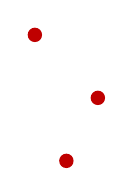
\begin{tikzpicture}[x=1cm,y=1cm]
  \dotrow{car P}{0.6}{9}{1.6}
  \dotrow{car Q}{1.4}{7}{0.8}
  \dotrow{car R}{1.0}{8}{0}
  \fill[red!75!black] (0.6,1.6) circle (2.6pt);
  \fill[red!75!black] (1.4,0.8) circle (2.6pt);
  \fill[red!75!black] (1.0,0) circle (2.6pt);
\end{tikzpicture}
\end{center}

\elem Think of the three cars starting a race together, so that the first dot in each row is laid at the same instant. Because $\tau$ is the same for all three, the \emph{second} dots (coloured red) are also laid at the same instant. Whichever second dot lies farthest from the start belongs to the car that covered the most track in that time, and covering more ground in the same time is what ``faster'' means. Q's second dot is farthest along, then R's, then P's. So
\[
\text{Q} > \text{R} > \text{P}.
\]
Notice that Q's row has the \emph{fewest} dots. That is irrelevant: the number of dots says how long the car was recorded, not how fast it went. Only the spacing carries speed.

\calc The gap between two neighbouring dots is the distance the car covers during one interval $\tau$. If the car's speed at time $t$ is $v(t)$, that distance is the integral of the speed over the interval,
\[
\text{gap} = \int_{t_0}^{t_0 + \tau} v(t)\,\dd t,
\]
which for a steady speed is simply $v\tau$. With the same $\tau$ in every diagram, a larger gap means a larger $v$, and the ranking follows: Q, then R, then P. The integral also explains the third rule above: if the diagrams had different $\tau$, a larger gap could come from a longer interval rather than a larger integrand.\qed
\end{example}

\begin{keyidea}[Dot spacing is speed]
For dot diagrams drawn with the same time $\tau$ between dots: the farther apart the dots, the faster the object. A fast object travels farther than a slow one in the time between dots. \elemtag\ Spacing $= $ speed $\times\ \tau$ when the speed is steady. \calctag\ Spacing $= \int v\,\dd t$ over one interval, always.
\end{keyidea}

\begin{example}{Counting gaps, not dots}{fencepost}
A dot diagram of a walker has eight dots with $\tau = \SI{0.25}{\second}$ and a spacing of \SI{0.45}{\metre} between neighbouring dots. (a) How much time does the diagram cover? (b) How far did the walker travel while it was being made? (c) What was the walker's speed?

\solution (a) Eight dots have only \emph{seven} gaps between them, and the time passes in the gaps: $7 \times \SI{0.25}{\second} = \SI{1.75}{\second}$. This is sometimes called a \emph{fencepost} error waiting to happen, because a fence with eight posts has seven panels. (b) Likewise the distance is seven gaps of \SI{0.45}{\metre}: \SI{3.15}{\metre}. (c) Speed is distance divided by time (Section~\ref{sec:speed} makes this precise): $\SI{3.15}{\metre}/\SI{1.75}{\second} = \SI{1.8}{\metre\per\second}$. Equivalently, one gap: $\SI{0.45}{\metre}/\SI{0.25}{\second} = \SI{1.8}{\metre\per\second}$, the same answer, because the walker's speed did not change. \calctag\ In calculus terms the whole-diagram calculation is $\int_0^{1.75} v\,\dd t = 3.15$, and dividing by \num{1.75} gives the \emph{average} speed; the one-gap calculation gives the average over a shorter stretch. They agree here because $v$ is constant.\qed
\end{example}

\begin{checkbox}
Does a dot diagram tell you which way the object was moving? A ball rolls from left to right at a steady speed and leaves a dot diagram; a second ball rolls from right to left at the same speed. Compare their diagrams.
\end{checkbox}

\subsection{When speed changes}

So far every diagram has had equally spaced dots, which is what a steady speed produces. Figure~\ref{fig:changing} shows what happens otherwise. A car pulling away from traffic lights covers more ground in each successive interval than in the one before, so its dots spread out. A car braking to a stop produces dots that bunch together. The direction in which the spacing changes is a direction along the diagram, and it tells you which way the car was going provided you know whether it was speeding up or slowing down.

\begin{figure}[htb]
\centering
\begin{tikzpicture}[x=1cm,y=1cm]
  \node[anchor=east] at (-0.3,1.6) {steady};
  \foreach \p in {0,1.5,3.0,4.5,6.0,7.5,9.0}{\fill (\p,1.6) circle (2.2pt);}
  \node[anchor=east] at (-0.3,0.8) {speeding up};
  \foreach \p in {0,0.3,0.9,1.8,3.0,4.5,6.3,8.4}{\fill (\p,0.8) circle (2.2pt);}
  \node[anchor=east] at (-0.3,0) {slowing down};
  \foreach \p in {0,2.4,4.5,6.3,7.8,9.0,9.9,10.5}{\fill (\p,0) circle (2.2pt);}
  \draw[->,>=Stealth,gray!70] (0,-0.5) -- (10.8,-0.5) node[right,font=\small,gray!90!black]{motion to the right};
\end{tikzpicture}
\caption{Three dot diagrams with the same $\tau$, all for motion to the right. Equal spacing means steady speed; spacing that grows means the object is speeding up; spacing that shrinks means it is slowing down. Chapter~2 studies the middle case in detail.}
\label{fig:changing}
\end{figure}

\begin{twoviews}{reading a changing speed from dots}
\elem Each gap is the distance covered in one interval $\tau$, so each gap divided by $\tau$ is the \emph{average speed during that interval}. A row of growing gaps is a row of growing average speeds. You cannot read the speed at a single instant from the dots, only the average over each interval; but the shorter you make $\tau$, the more nearly ``the average over an interval'' becomes ``the speed at an instant.''

\calc If $x(t)$ is the object's position along the track, the $n$th gap is $x(n\tau) - x((n-1)\tau) = \int_{(n-1)\tau}^{n\tau} v(t)\,\dd t$. Dividing by $\tau$ gives the mean value of $v$ over that interval. As $\tau \to 0$ the mean value tends to $v$ at the instant, which is the derivative $\dd x/\dd t$: a dot diagram with a very short $\tau$ is a numerical picture of the derivative of $x(t)$. Section~\ref{sec:instant} returns to this.
\end{twoviews}

\subsection{Making dot diagrams in the laboratory}

A traditional school apparatus makes dot diagrams directly. A long strip of paper tape is attached to the back of a cart. As the cart moves, the tape is dragged under a \emph{ticker timer}, a small device whose vibrating arm strikes the tape through a disc of carbon paper at a fixed rate, typically fifty times per second. Every strike leaves a dot. When the cart stops, the tape carries a dot diagram of its entire journey with $\tau = \SI{0.02}{\second}$. (Photographed with a phone at a known frame rate, a moving object gives the same thing without the tape; Exercise~\ref{ex:phone} asks you to try it.)

The ticker timer makes the three rules of Definition~\ref{def:dotdiag} concrete. If you slow the timer so that it strikes less often, the cart moves farther between strikes and the dots spread out, even though the cart is going no faster. If you want to compare a fast cart with a slow one, the timer must strike at the same rate for both. And if the cart is speeding up, the timer must \emph{not} speed up with it: a timer that struck faster and faster would compress the growing gaps, and you could no longer tell how much of the pattern was the cart and how much was the timer.

\begin{checkbox}
A ticker timer is set to strike \num{50} times per second. A cart pulls the tape through it, and a student measures the first ten gaps as (in \si{\centi\metre}) 1.6, 1.6, 1.6, 1.6, 1.6, 1.9, 2.2, 2.5, 2.8, 3.1. Describe the cart's motion in words, and give its speed during the first five intervals.
\end{checkbox}
